\chapter{真实大规模场景数据下的混合隐式场学习}
\section{基于时间-位姿隐式场的多元传感信息配准}
大规模场景的混合隐式表达对于真实场景中地图重建是自动驾驶、无人机运输等智能交通应用的下一代地图表征工具。然而对于大规模场景的多元传感数据的同步采集,现有的同步RGB-D相机因其可以感知到的深度范围及其有限,从而不能被直接应用,而使用不同步的RGB相机和深度传感器(激光雷达等)不可避免的需要解决其中的时钟同步问题。受近期的自动标定相机内外参数的的神经隐式场方法所启发,在本节中,我们提出了首个自动标定RGB相机和深度传感器间采样频率和偏置的解决方案。

我们利用了一个重要的领域先验,即同时搭载不同种类传感器的数据采集设备在时空上覆盖了几乎完全相同的行动轨迹,提出建模时间到位姿的隐式函数关系。我们的方法可以作为第\ref{chapter: omninerf}章中混合隐式场景表示模型的前置网络,提供较为准确的位姿数据。

\subsection{简介}
近年来,神经隐式表达被广泛用于大规模场景的隐式重建中\cite{tancik_block-nerf_2022, rematas_urban_2022, turki_mega-nerf_2022, xiangli_bungeenerf_2022},由于此类方法通常具有较好的新视角渲染能力,他们通常被看作下一代视觉导航系统中的地图表示模型。我们不妨想象,在未来,同时定位与建图(Simultaneously Localization and Mapping, SLAM)系统可以快速整合不同种类的传感信息,构建准确的基于神经隐式场的地图表示\cite{zhu_nice-slam_2022, zhu_nicer-slam_2023, sandstrom_point-slam_2023},场景图(SceneGraph)算法可以通过车端RGB相机和消费级激光雷达快速构建周边区域的动态场景图,准确对路端中行人、机动车的未来轨迹进行预测\cite{ost_neural_2021, kundu_panoptic_2022, yang_urbangiraffe_2023, , chen_geosim_2021}。

然而,目前的这些方法仍然没有系统性地解决使用深度数据作为有效监督信号的一个关键问题。使用深度图作为监督信号加入到神经隐式表达的训练过程听起来是一个非常浅显易懂的概念,然而这一概念在真实大场景数据获取、使用上存在着相当复杂的时间同步问题。我们注意到市面上使用较为广泛的RGB-D同步相机如微软Kinect相机\cite{zhang_microsoft_2012}、英特尔RealSense相机\cite{, zabatani_intel_2020}等通常只能感知到受限范围内(通常在5米以内)的物体,从而只能用于室内场景的数据获取中,而不能用于更加广泛的室外场景自动驾驶、无人机运输等智能交通算法中。 另一方面,使用异步的 RGB 和深度传感器会带来更多的复杂性,因为这通常意味着我们需要估计每个RGB帧和深度帧之间的转换矩阵。

\begin{figure}[ht]
    \centering
    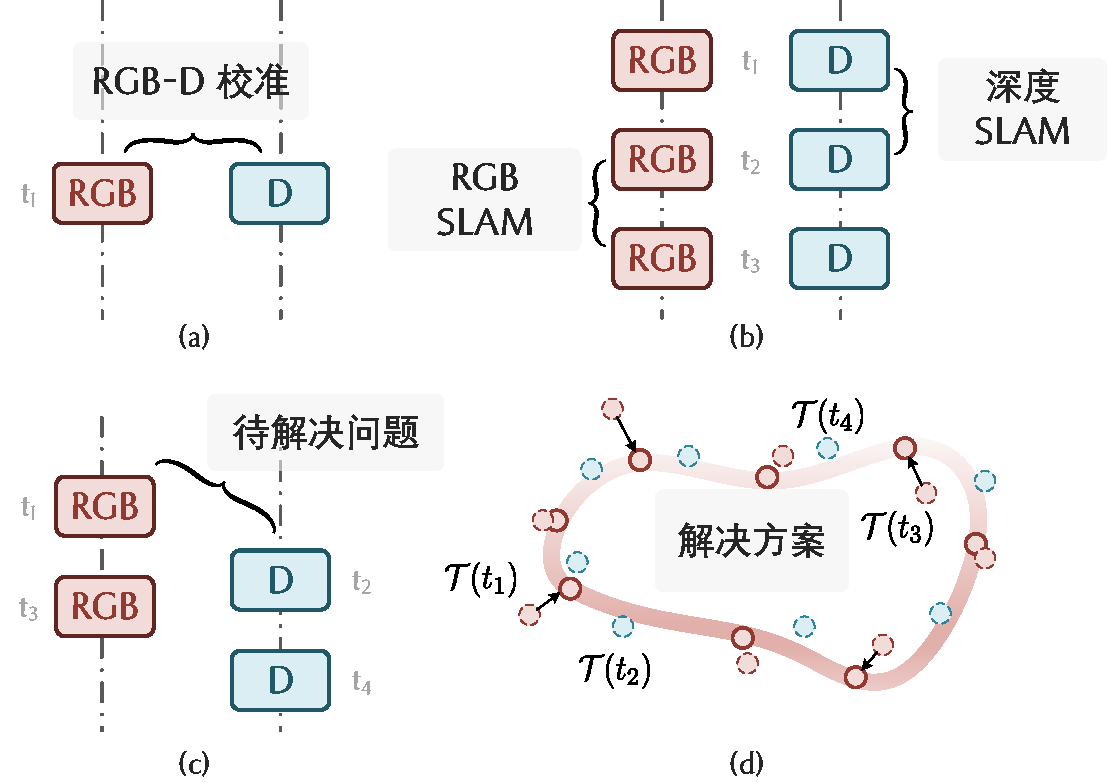
\includegraphics[width=0.8\textwidth]{undergraduate-thesis/images/time-pose function/teaser.pdf}
    \caption{我们感兴趣的问题与其他现有问题之间的比较的示意图。}
    \label{fig: time-pose function teaser}
\end{figure}

我们将我们感兴趣的问题与图\ref{fig: time-pose function teaser}中广泛关注的其他现有问题进行比较:
\begin{enumerate}
    \item [(a)]RGB-D 校准方法\cite{jeong_self-calibrating_2021, bian_nope-nerf_2022}估计深度相机和 RGB 相机之间的变换关系,即内参数矩阵,此类方法通常使用点对点的配准方法来实现;
    \item [(b)] 给定连续获取的 RGB 或深度图,基于 RGB 的 SLAM\cite{campos_orb-slam3_2021, mur-artal_orb-slam_2015, engel_direct_2018, zhu_nicer-slam_2023}和基于深度的 SLAM \cite{niesner_real-time_2013, xu_multi-scale_2018}则估计相邻帧之间的转移矩阵 $\{T_{ij}\}$;
    \item [(c)] 我们感兴趣的问题则是通过从 RGB 序列的时间戳所对应的位姿序列中,学习其中隐含的轨迹先验来估计深度序列的相机轨迹$\{T_i^d\}$。
\end{enumerate}

\begin{figure}[t]
    \centering
    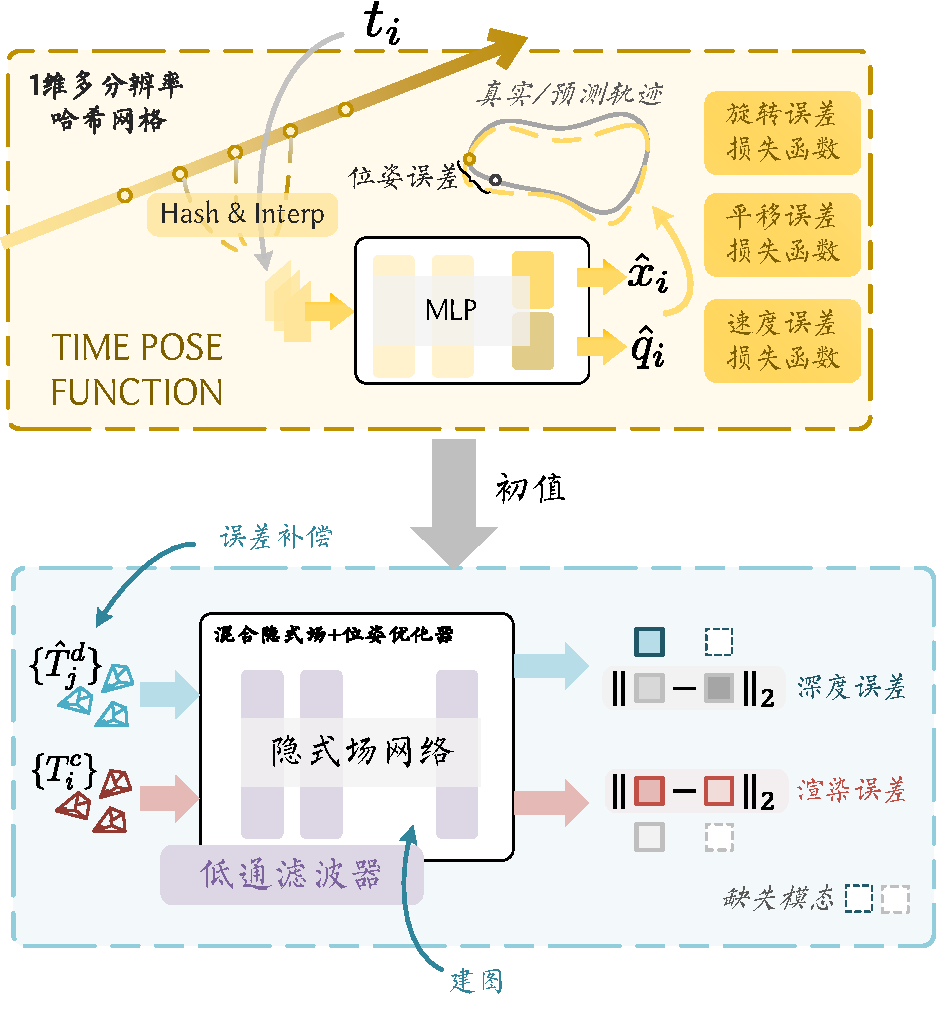
\includegraphics[width=0.8\textwidth]{undergraduate-thesis/images/time-pose function/main_export.pdf}
    \caption{系统概述图。我们的系统优化过程可以分为两个阶段。在第一阶段,TPF从 RGB 序列中时间和相机位姿之间的隐式函数关系中学习未知的深度相机位姿。在第二阶段,优化器同时训练具有深度监督的混合场景表示,并对估计的深度相机位姿进行精调。}
    \label{fig:time-pose function main figure}
\end{figure}

在本节中,我们受到近期将神经辐射场与相机内外参数同时优化的方法\cite{yen-chen_inerf_2021, lin_barf_2021, bian_nope-nerf_2022}的启发,我们希望在时空不同步的RGB-D序列中同时恢复隐式场和相机位姿的方法。我们注意到这个问题存在一个自然的解决方案:
\begin{quote}
    将 RGB 和深度帧分别处理为在某些时间戳处具有\textbf{缺失模态}的相机捕获的帧。
\end{quote}

因此,以前的方法如 BARF\cite{lin_barf_2021} 可以很容易地扩展到这种情况,即在优化开始阶段为相机内外参任意赋予一个初始值,并在优化过程中通过反向传播算法不断调整。然而,这种基线方法未能在此问题中利用有用的特定领域先验,即RGB和深度相机实际上经过相同的连续运动轨迹。

为此,我们提出使用一种新型的时间-位姿隐函数(Time-Pose Function, TPF)对此先验进行建模,TPF将时间戳映射到六自由度相机位姿。就像神经符号距离场或辐射场中对具有 3D/5D 输入的函数进行逼近的方式一样, TPF逼近一个将 1D 时间戳作为输入并输出 SE(3) 流形\cite{sola_micro_2021}中的变换的函数。换句话说,这个TPF也是一个隐式场。我们将它与前文提到的混合隐式地图结合起来,形成如图\ref{fig:time-pose function main figure} 所示的级联架构。因此,在该框架下进行优化可以同时构建用于建图的城市规模混合隐式场,并校准 RGB-D 帧之间的不匹配问题。

\subsection{相关工作概要}
\textbf{神经隐式表达:}
通过每个圆锥太体覆盖的体积的集成位置编码 (IPE) 表示,MipNeRF\cite{barron_mip-nerf_2021}有效地渲染视锥(而不是射线),从而减少了混叠的伪影现象。 NeRF++\cite{zhang_nerf_2020}分别对前景和背景表示进行建模,并分别进行采样,以应对无界 3D 场景建模的挑战。 NeRF-W\cite{martin-brualla_nerf_2021}引入了外观和瞬态编码来弥补受可变光照或瞬态遮挡物影响的弱点。 InstantNGP\cite{muller_instant_2022} 采用具有可训练特征向量的多分辨率哈希表,使 NeRF 能够学习高质量的神经图形基元。

Block-NeRF\cite{tancik_block-nerf_2022}和 Mega-NeRF\cite{turki_mega-nerf_2022} 在空间上将场景分解为单独训练的 NeRF,使场景表示能够扩展到任意大的环境。 Bungee-NeRF\cite{xiangli_bungeenerf_2022}使用多尺度数据模型,在该模型中,可以在卫星级别的截然不同的尺度上观察到图像的变化。通过引入 LiDAR 和天空建模并补偿不同的曝光,城市辐射场\cite{rematas_urban_2022}扩展了 NeRF 模型以产生令人印象深刻的 3D 表面重建并在室外环境中合成高质量的新颖视图。

此外,借助多视图立体几何\cite{deng_depth-supervised_2022} 或深度先验信息\cite{roessle_dense_2022} 的密集深度监督,NeRF 在新颖的视图合成和深度预测方面取得了惊人的成果,但难以扩展到大规模户外场景.

\textbf{相机标定:}
当前有多种 SLAM 系统通过联合估计相机参数和 3D 几何形状来重建场景。 ORB-SLAM\cite{mur-artal_orb-slam_2015}通过关联特征对应关系实时重建场景和估计相机位姿。 SfM(Structure-from-Motion,运动恢复结构) 系统\cite{schonberger_structure--motion_2016, chen_uncertainty-driven_2023} 能够同时校准内部和外部相机参数并重建场景。 相机-雷达混合SLAM\cite{kong_vmap_2023, deng_nerf-loam_2023} 对齐相机中心周围单位球体中的点和视觉特征之间的对应关系,从而提高了位姿估计精度并减少标定时间。

随着基于 NeRF 的 3D 场景重建和渲染研究的蓬勃发展,最近的工作估计了 NeRF 之上的相机参数。给定一个经过训练的 NeRF 模型,iNeRF\cite{yen-chen_inerf_2021} 能够根据观察到的图像和来自 NeRF 模型的渲染图像之间的光度损失,执行无网格、仅 RGB 的 6-DOF 位姿估计。由于 RGB 和深度的时间一致性,iMAP\cite{sucar_imap_2021} 和 NICE-SLAM\cite{zhu_nice-slam_2022} 在房间内实时进行高保真重建和位姿估计方面取得了显著成果。 Martin-Brualla 等人提出了结合 TSDF 和辐射场的混合隐式场\cite{azinovic_neural_2022},在优化相机位姿的同时提高了外观和几何形状的整体重建质量。与基于 NeRF 的方法不同,NeRFmm \cite{wang_nerf--_2022},NopeNeRF\cite{bian_nope-nerf_2022} 和 SCNeRF \cite{jeong_self-calibrating_2021} 在训练中联合优化相机位姿和内在函数。 NeRFmm\cite{wang_nerf--_2022}只能用于前向场景。 SCNeRF\cite{jeong_self-calibrating_2021} 适用于具有任意非线性失真的通用相机。两者都不能扩展到大规模场景,不适用于本文中RGB-D错配场景的设置。


\subsection{研究动机与问题描述}
问题。我们的目标是像 Mega-NeRF\cite{turki_mega-nerf_2022} 或 BungeeNeRF\cite{xiangli_bungeenerf_2022} 等先前工作中所做的那样,学习用于大规模场景表示的神经隐式场,这对于城市规划或机器人模拟等新兴应用至关重要。然而,这些先前的工作未能利用激光雷达等深度传感器捕获的几何信息。该问题现在已经收到了研究社区较大的关注\cite{deng_depth-supervised_2022,roessle_dense_2022},因为它可用于训练具有快速收敛性的无漂浮物 NeRF。为此,我们想解决在训练大规模隐式场时使用深度监督的问题。

\textbf{挑战:}
这个问题的基本挑战之一是异步 RGB-D 数据。据我们所知,没有用于大型场景的易于访问的同步 RGB-D 传感器套件(如 RealSense 或 Kinect),并且根据时间戳简单地同步它们无法完全解决错位问题。我们没有将它们与昂贵的硬件严格同步,而是从算法的角度来看。这是一个新的自校准设置:在训练大规模 NeRF 的同时在线校准 RGB-D 相机变换。

\textbf{输入:} 在使用航空图像进行大规模场景建模的许多先前工作的基础上\cite{turki_mega-nerf_2022,xiangli_bungeenerf_2022},我们假设无人机捕获的输入 RGB-D 流:一组 RGB 相机图像$\{\mathcal{I}_i\}_{i=1}^{N_c}$和一组深度图$\{\mathcal{D}_i\}_{i=1}^{N_d}$。由于异步情况存在,这两个流在概念上如图\ref{fig: time-pose function teaser}-c所示,我们的目标是恢复它们之间的时空转换。鉴于我们的重点是相对变换,在不失一般性的情况下,将 RGB 或深度的位姿作为参考点都是可行的。为方便起见,我们假设彩色图像的相机位姿是通过 SfM 算法获得的,来预测深度图位姿。

\textbf{输出}:我们的最终目标是训练一个准确的神经隐式表示,在给定的视角$\mathbf{T}$下输出逼真的 RGB 图像$\hat{\mathcal{I}}$以及准确的深度图 $\hat{\mathcal{D}}$。同时,我们校准未知的深度相机位姿$\mathbf{T}_i^d$ 有助于引入深度监督以获得更好的场景表示。

\textbf{优化过程:}
为了利用隐式时间-位姿函数关系,我们建议使用基于回归的模型,该模型将 1D 时间戳作为输入并输出相应的 6-DOF 相机位姿。在实践中,我们使用 RGB 图像位姿来训练隐式时间位姿函数并在模型收敛后预测深度位姿。然而,时间关系本身可能无法为基于 NeRF 的神经渲染器提供足够的准确性,这需要像素级的准确性来构建逼真的场景图。因此,在第二阶段,我们在 NeRF 训练过程中同时优化最初预测的深度位姿,其中 RGB 和深度图像都用作监督信号。正如我们稍后在实验中所证明的那样,使用纯 RGB 监督优化神经隐式场足以实现照片般逼真的渲染;然而,学习到的场景几何可能无法满足真实世界的机器人应用需求。引入具有原始深度位姿对齐的深度传感监督甚至可能会损害准确性。为了利用无人机在同一轨迹上捕获 RGB 图像和深度图的先验,我们对 RGB-D 帧的时间戳$\{t_i\}_{i=1}^{N_c+N_d}$ 进行建模,并且相应的相机内在函数也取自EXIF 信息作为算法输入。

\begin{figure}[ht]
    \centering
    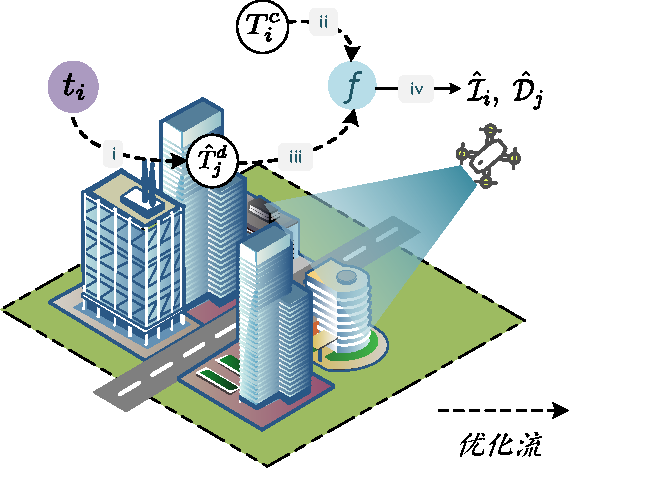
\includegraphics[width=0.6\textwidth]{undergraduate-thesis/images/time-pose function/Problem Formulation export.pdf}
    \caption{优化流程图}
    \label{fig:time-pose function optimization flow}
\end{figure}

\subsection{时间-位姿隐式轨迹函数 (TPF)}
在这一部分中,我们介绍了估计相机位姿的时间位姿函数 $\mathcal{T}$。我们将相机轨迹表示为隐式时间位姿函数,其输入是时间戳$t$,输出是 6-DoF 相机位姿。位姿输出由一个 3-D 平移向量 $x_i$ 和表示为四元数\cite{sola_micro_2021} $q_i$ 的 4-D 旋转向量组成。
\begin{equation}
    \mathcal{T}:\quad t_i\to\mathbf{T}_i=[x_i, q_i]
\end{equation}

我们将TPF函数用一个一维多分辨率哈希网格 $\{G^{(l)}\}_L^{l=1}$ 近似,输出的参数会用一个浅层多层感知机解码器$\mathcal{F}_\Theta$解码。哈希网格由 $L$ 级独立的特征网格组成。当为所有时间戳范围内的任意时间戳 $t_i$ 查询相机位姿 $\mathbf{T}_i$ 时,我们从每个网格层采样哈希编码并对提取的编码后通过二次插值并连接在一起以获得特征向量 $\mathcal{V}_i$。获得内插特征向量后,使用共享 MLP 处理特征 $\mathcal{V}_i$,然后将其输出馈送到两个分离的全连接层,以分别预测输出平移 $x_i$ 和旋转 $q_i$ 向量。网络前传过程可以用以下等式表示:
\begin{align}
    \mathcal{V}_i&=\mathcal{F}_\Theta(\mathtt{concat}\{\mathtt{interp}(h(t_i;\pi_l), \mathcal{G}_\theta^l)\}^L_{l=1}),\\
    \hat{\mathbf{T}}_i &= [\hat{x}_i, \hat{q}_i] = l_{trans}(\mathcal{V}_i; \Theta_{trans}), l_{rot}(\mathcal{V}_i; \Theta_{rot}),
\end{align}
其中$\mathtt{interp}$表示插值算子,$h$是由$π_l$参数化的哈希函数,$l_{trans},l_{rot}$是两个全连接层,其中$\Theta_{trans},\Theta_{rot}$分别表示网络参数。

由于深度图和 RGB 图像都是由同一架无人机在同一飞行中收集的,因此除了两个传感器在飞机上的位置不同外,它们在时间和空间方面的轨迹几乎相同。因此,我们可以使用我们从 RGB 序列中学习到的隐式时间-位姿函数直接预测对应于深度序列时间戳的位姿,以及传感器位置之间已知的位姿变换 $\mathbf{T}_\text{sensor}$。


\subsection{优化TPF模型}
表示用于优化相机位姿的旋转的最常见选择是旋转矩阵\cite{yen-chen_inerf_2021}或 欧拉角。然而,由于它们与 SO(3) 的非同胚表示空间,它们在表示旋转时不是连续的\cite{kendall_posenet_2015}。我们选择使用单位四元数作为我们的原始表示,因为任意 4-D 向量可以通过将它们归一化为单位长度轻松映射到合法的旋转。

为了优化时间-位姿函数,我们提出了以下目标函数:
\begin{equation}
    \mathcal{L} = \lambda_{trans}\mathcal{L}_{trans}+\lambda_{rot}\mathcal{L}_{rot}+\lambda_{speed}\mathcal{L}_{speed},
\end{equation}
其中,$\lambda_{trans}, \lambda_{rot}$会随着训练过程自动调整。我们将在后文介绍自适应权重。

\textbf{位移和旋转矢量的直接优化:}
我们通过评估估计相机位姿和地面实况相机位姿的均方误差 (MSE) 直接优化欧几里得空间中的平移和旋转向量:
\begin{align}
    \mathcal{L}_{trans} &= \text{MSE}(\{x_i\}, \{\hat{x}_i\})\\
    \mathcal{L}_{rot} &= \text{MSE}(\{q_i\}, \{\hat{q}_i\})
\end{align}

由于 $x$和 $q$ 的单位不同,因此比例因子 $\lambda_{trans}$ 和 $\lambda_{rot}$ 在平衡损失方面发挥了重要作用。为了防止平移和旋转在训练中相互产生负面影响并利用可能的相互促进作用,我们通过使用同方差不确定性 \cite{kendall_geometric_2017} 使加权因子可学习:\begin{equation}
    \mathcal{L}_{\sigma} = \mathcal{L}_{trans} \exp(−\hat{s}_{trans}) + \hat{s}_{trans} + \mathcal{L}_{rot} \exp( −\hat{s}_{rot}) + \hat{s}_{rot},
\end{equation}
其中 $\hat{s}$ 是可学习的,因此损失项会自动平衡。手动选择权重需要不断调整参数,但可以获得相似的性能。

\textbf{移动速度的梯度优化:}
观察到时间-位姿函数本质上是位移和角位移相对于时间的函数,我们可以使用平均线速度来监督网络输出相对于输入向量的梯度。这里平均速度是指从当前帧和相邻两个帧的地面真值相机位姿计算的平均值,而不是整个序列中的平均值。由于在无人机拍摄的场景中线速度变化较小,角速度变化相对较大,因此仅使用平均线速度来监督神经网络,而后者在我们的设置中没有受到监督:
\begin{equation}
    \mathcal{L}_{speed} = \text{MSE}(\{\frac{x_i-x_{i-1}}{t_i-t_{i-1}}\}, \{\hat{v}_i\})
\end{equation}

\subsection{后端优化与TPF误差补偿}
虽然时间-位姿函数为建图阶段提供了一个很好的深度相机位姿初始值,但在一些离群帧中仍然存在明显的错误。我们将描述如何同时执行映射和位姿优化,以补偿时间-位姿函数的误差。

对于地图表示,我们使用第\ref{chapter: omninerf}章所提出的混合隐式表达。在此基础指上,我们联合优化不准确的相机位姿和隐式映射:当优化场景表示参数 $\Theta_{Map}$ 时,估计的深度相机位姿 $\hat{\mathbf{T}}_i \in SE(3)$(其中 $t \in \mathbb{R}^3$, $q \in SO(3)$)将在流形上同时优化这些参数:
\begin{equation}
    \hat{\Theta}_{Map},\hat{\mathbf{T}} = \arg\min\mathcal{L}(\mathbf{T}, \Theta_{Map} | \mathbf{T}_0, \{\mathcal{I}_i\}, \{\mathcal{D}\}),
\end{equation}
其中 $\mathcal{L}$ 是目标函数,$\mathbf{T}_0$ 是时间-位姿函数的预测值。

为了补偿时间-位姿函数提取位姿的误差,我们通过应用一组可训练的位姿校正项进一步优化估计值。受 BARF\cite{lin_barf_2021} 的启发,在解决位置校准问题时,低频信号可以预测比高频信号更一致的位移,这很容易导致次优优化结果。传统 NeRF 渲染中的位置编码在高频细节方面显着改善了合成视图。使用可以削弱位置编码效果的低通滤波器将具有与平滑类似的效果。因此,在联合优化阶段中使用动态低通滤波器来帮助优化不准确的深度帧位姿。

\newpage
\section{退化真实输入数据下的准确场景表示学习}
在上一节中,我们介绍了如何配准不对齐的RGB-D序列,这一方法可以在真实场景中有效地融入深度信息。然而,我们在真实实验过程中同样发现,面对雾天、雨天等退化天气情况时,由于深度传感器本身受影响较大,因而我们不能获得较为准确的传感器数据。然而另一方面,我们发现类似雾天这样的由于散射介质引起的图片退化可以从另一方面提供物体的深度信息。

因此在本节中,受最近对从退化(例如,嘈杂或模糊)图像中学习隐式场的研究兴趣激增的启发,我们研究从模糊带雾图像中学习隐式场的问题。一个有趣的事实是,许多以前的方法侧重于避免不存在的漂浮物(通常指渲染出来的瑕疵),而在本课题中,我们希望通过建模\textbf{真正}的漂浮物来简介获得深度信息。我们首先证明,从模糊图像中学习的隐式场不能用于渲染可靠的深度,这与通过光衰减的雾度有关。为此,我们分析隐式场了学习到的体积密度值的分布,构建了一个加权函数,并证明了该函数可用于生成可信的深度图。同时,我们引入了协方差损失,用于消除颜色衰减和视点相关隐式之间固有的歧义。最后,我们通过编辑隐式场中的漂浮物密度来开发雾度处理管线。

\subsection{简介}
新视图合成的最新进展利用神经辐射场来恢复复杂的场景几何和外观。由单个多层感知器参数化为场景坐标和相应场景量之间的映射函数,可以以自监督的方式从构成的多视图图像中学习隐式表示。优化的关键是体积渲染技术,该技术将像素值视为沿来自相机接收到的表面点的射线的辐照度的积分,从而保证光度误差反向传播到神经场。这种模式在大多数情况下都能很好地呈现照片级逼真度的新视图渲染结果。

然而,大气中的悬浮颗粒,或者换句话说,漂浮物,会导致图像退化。这种现象在室外场景中非常常见(如雾天、霾天或烟雾等),他们主要由大气中漂浮物所产生的散射现象导致。这种模糊图像的退化导致相机接收到的辐照度减弱。这对从模糊图像中学习辐射场提出了挑战,因为在这种衰减的情况下,光度一致性不再成立。由于场景辐射和雾度之间固有的歧义,从模糊图像中监督场景的辐射场会导致嘈杂的几何形状和外观,如图所示。

\begin{figure}[ht]
    \centering
    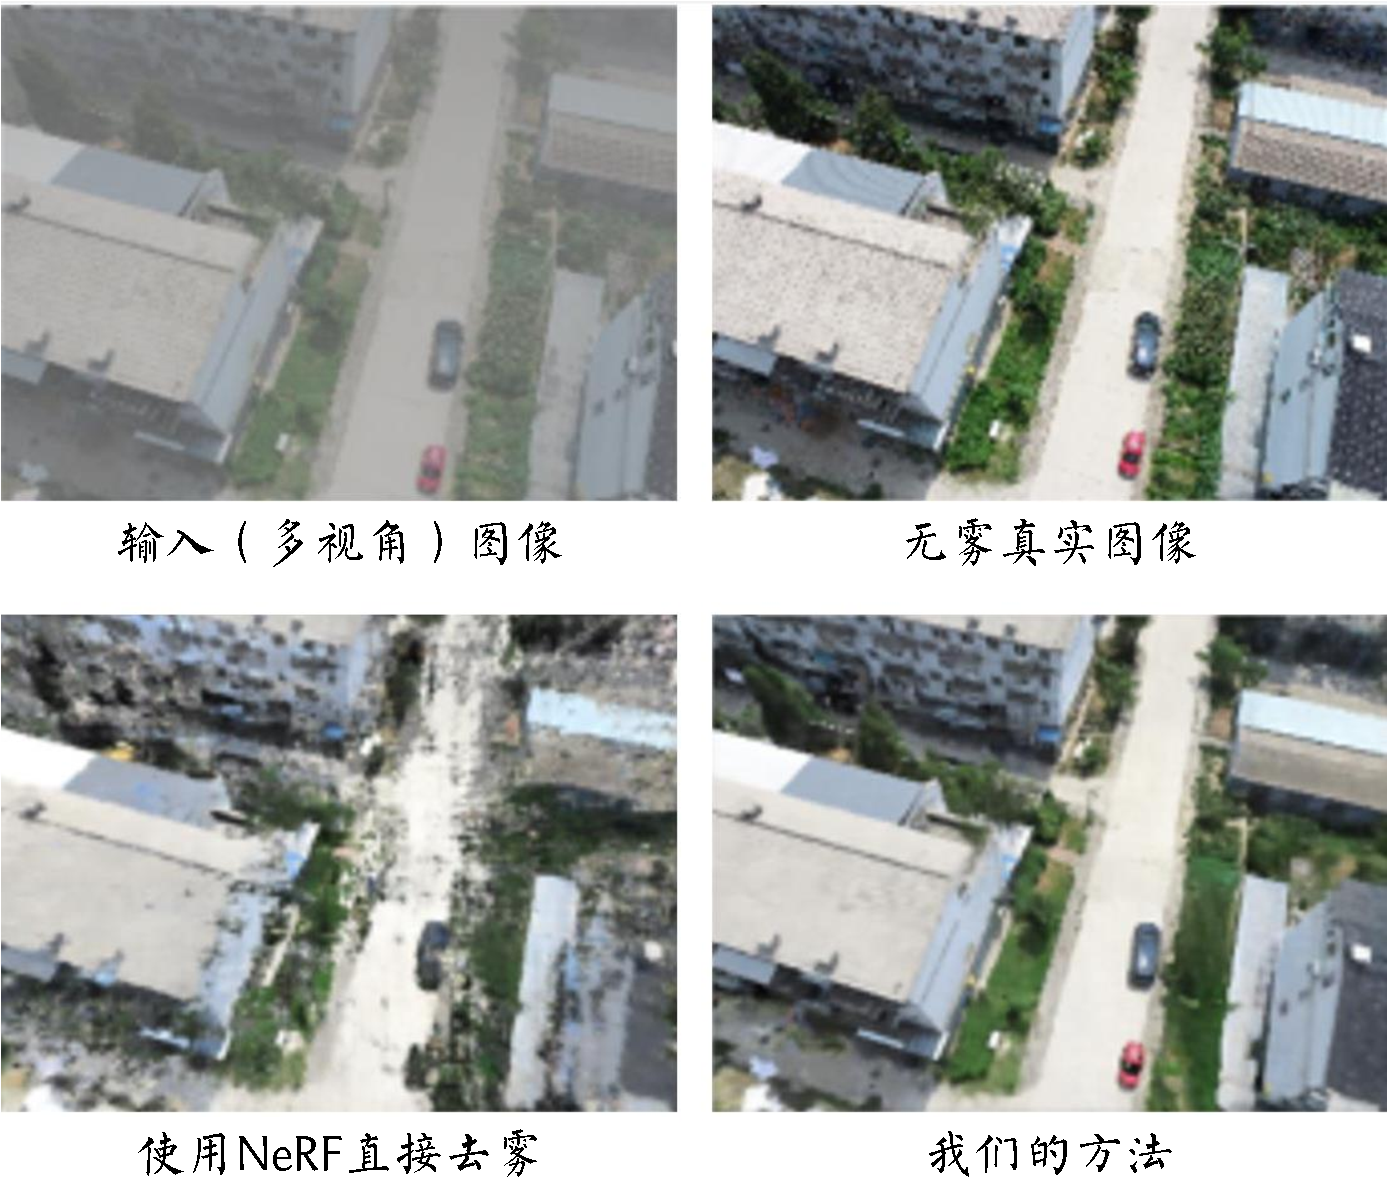
\includegraphics[width=0.8\textwidth]{undergraduate-thesis/images/dehazing-nerf/teaser.pdf}
    \caption{使用退化带雾图像进行多视角去雾。}
    \label{fig:dehazing-nerf teaser}
\end{figure}

通过分析辐射场内自然学习到的密度分布,我们首先深入探讨了漂浮物如何影响体积渲染过程的问题。从几何学上讲,漂浮物会导致地表前方的密度非零,因此渲染的深度图像会出现偏差,而从光度方面来看,由于传输依赖于深度,在不同距离观察朦胧场景可能会导致不同的结果即使场景辐射场与视图无关,视点之间的退化行为同样如此。这种有偏见的深度推理和模棱两可的视图依赖性导致辐射场的学习难以处理。为了解决这些问题,我们提出了一种改进的深度图细化平均权重。就视图依赖性歧义而言,我们引入了一个基于协方差的正则化项,以减小辐射和雾霾引起的辐照度衰减之间的强耦合。这些方式保证了无雾场景表示的准确恢复以及漂浮物的浓度控制。

\subsection{相关工作概要}
\textbf{图像去雾:}
现有去雾方法大致可以分为三类:基于先验的方法、基于学习的方法和散射介质中的 3D 重建:
\begin{enumerate}
    \item \textbf{基于先验信息的去雾方法}。基于先验的方法依赖于物理散射模型,通过使用启发式先验来估计和去除雾霾,这些先验包括对比度最大化先验、暗通道先验、颜色衰减先验、强度框先验和非局部先验 \cite{kaiming_he_single_2009, nishino_bayesian_2012, fattal_dehazing_2015, wu_contrastive_2021}。虽然这些方法产生了视觉上逼真的结果,但所采用的先验仅限于特定场景。例如,当图像中没有天空区域时,之前的暗通道方法表现不佳\cite{kaiming_he_single_2009},因为它依赖于该区域的 RGB 值来估计大气光。此外,由于先验是在图像域中指定的,因此可能无法完全保证多视图一致性。
\end{enumerate}

\subsection{散射介质的理论模型}

\subsection{研究动机与方法描述}

\subsection{处理视角相关-颜色二义性}